% !Tex root = main.tex

% least laxity first

% 


\chapter{Návrh riešenia}
% V tejto kapitole vysvetľujeme ako prebieha komunikácia medzi agregátorom a systémovým operátorom v našom navrhovanom modeli. Taktiež rozoberáme, ako prebieha triedenie a iné operácie, ktoré sa vykonávajú v našom navrhovanom modeli.
V tejto kapitole predstavujeme návrh modelu práce agregátora. Modelom práce agregátora rozumieme spôsob ako agregátor dodáva energiu elektromobilom. Agregátor používa algoritmy v tejto kapitole na riešenie optimalizačného problému [..odkaz]. 
% V tejto kapitole popisujeme navrhnuté riešenie optimalizačného problému dodania maximálneho množstva požadovanej energie elektromobilom pri zachovaní obmedzení infraštruktúry nabíjacej siete.
% mam specifikovat co presne som pridal???



% \section{Problém nájdenia optimálneho plánu nabíjania.}
% % \subsection{Scheduling algoritmy.}
% Problém nájdenia optimálného plánu nabíjania elektromobilov je optimalizačným problémom. Existuje veľa spôsobov riešenia optimalizačného problému, nájdenia optimálneho plánu nabíjania vozidiel, keďžE môžeme použiť kontrolné algoritmy alebo jednoduché scheduling algoritmy. Kontrolné algoritmy MPC a PPC riešia problém nájdenia optimálneho plánu tým, že predikujú údaje o budúcich príchodoch elektromobilov. Algoritmus PPC sa používa v kombinácii s jednoduchým plánovacím algoritmom. 

% Vstupom všetkých scheduling algoritmov je množina elektromobilov a parametre na strane agregátora flexibility. Výstupom všetkých scheduling algoritmov je plán nabíjania (scheduling). \cite{shcedulingdetailexplanbook} 


% zda sa ze preklad offline a online dobry neexistuje a dost ludi ho pouziva

% TODO: vysvetlit co je online algoritmus tu alebo vyssie?

% odkaz na vetu ze je vylepsenim
\section{Smoothed Least Laxity First.}
Algoritmus Smoothed Least Laxity First (skrátene sLLF) vznikol v reakcii na oscilácie v nabíjaní elektrických vozidiel pomocou algoritmu LLF. Oscilácie v nabíjaní elektromobilov skracujú životnosť niektorých baterií elektrických vozidiel (napr. batéria L-ion). Nabíjanie elektrických vozidiel pomocou algoritmu sLLF už neobsahuje oscilácie.

% asi to mali byt prudke oscilacie a nie len oscilacie, pozriet na to este 

% Algoritmus sLLF je algoritmus určený pre nabíjanie elektromobilov v nabíjacej stanici. 

Algoritmus sLLF rozhoduje o aktuálnom pláne nabíjania elektromobilov na základe infomácii do aktuálneho času (sLLF je online algoritmus). Algoritmus sLLF pre každý časový krok $k \in K$ maximalizuje minimálnu laxitu a tým zväčšuje rozpätie možných rýchlostí nabíjania. aktuálne nabíjaných elektrických vozidiel pre budúci časový krok v diskrétnom modeli. \cite{lee2021adaptivephd}



Laxitou popisujeme v algoritme sLLF flexibilitu (urgenciu) nabíjania. Laxitu $l_{i}(k)$ elektromobilu $i$ v čase $k$ definujeme takto:
% pouzivajme ucelene jedno pismenko na urcenie casu, napr k
\begin{align}
    l_{i}(k) = \begin{cases} 
    \left[d_{i} - k\right]^{+} - \frac{e_{i}(k)}{\overline{r}_{i}} & k \geq a_{i},\\
    +\infty & k < a_{i},
 \end{cases}
\end{align}
kde $\overline{r}_{i}$ je maximálna rýchlosť nabíjania elektromobilu $i$. $\left[x\right]^{+}$ je projekcia $x$ do množiny nemínusových reálnych čísel $R_{+}$.


% TODO: preloz listing nazov do slovenciny

% Get active EVs
% Calculate laxity for each EV and store them:

% jedno z rieseni, je nepisat komentare do kodu ale mimo kod
% \begin{lstlisting}[caption={My Caption},captionpos=b,mathescape=true]


% \begin{end}
Online algoritmus sLLF v každom kroku $k \in K $ rieši optimalizačný problém:
\begin{align}
    \underset{r(k)}{max} \sum_{i \in V_{k}}^{} \overline{r}_{i} f(l_{i}(t + 1)) \\
    \text{subject to:} \eqref{basic-constraints:subeq1}, \eqref{basic-constraints:subeq2},\eqref{basic-constraints:subeq3}
\end{align}

Riešením optimalizačného problému (odkaz) je:

\begin{align}
r^{*}_{i}(t) = [\overline{r}_{i}(L(t) - l_{i}(t) + 1   )]_{0}^{min(\overline{r}_{i}, e_{i}(t))},
\end{align}
$[x]_{a}^{b}$ je projekcia na interval 


\begin{lstlisting}[caption={Pseudokód online algoritmu sLLF.},captionpos=b,mathescape=true]
for $k \in K$ do:
    $V_{t} := \{i | a_{i} \leq t < d_{i} \land e_{i}(t) > 0\}$
    $Lax_{t} := \{l_{i}(t), i \in V_{t}\}$
    $l_{L} := min(Lax_{t}) - 1$
    $u_{L} := max(Lax_{t})$
    while $|u_{L} - l_{L}| \geq \epsilon$ do
        $L(t) := \frac{u_{L} + l_{L}}{2}$
        if $\sum_{i \in Vt} [\overline{r}_{i}(L(t) - l_{i}(t) + 1)]_{0}^{min(\overline{r}_{i}, e_{i}(t))} \leq P(t)$ then
            $l_{L} := L(t)$
        else
            $u_{L} := L(t)$
    $r^{*}(t) := \{[\overline{r}_{i}(L(t) - l_{i} + 1)]_{0}^{min(\overline{r}_{i}, e_{i}(t))}, i \in V_{t} \}$


\end{lstlisting}



\section{Penalised Predictive Control.}
% \section{Penalised Predictive Control.}



% popisat cely ten problem
% co je closed loop algorithm

% lepsie je tam dat aj cisla riadkov kodu do obidvoch prikladov
% popisat co systemovy operator optimalizuje


% odstranit listing nazov
\begin{lstlisting}[caption={Pseudokód koordinácie agregátora a systémového operátora.},captionpos=b,mathescape=true]
    for $k \in K$:
        $u_{t} = \phi_{t}(p_{t}) = min ...$
        $C_{t} = C_{t - 1} + c_{t}(u_{t})$

        $e_{t}(i) = e_{t - 1}(i) - s_{t}(i), \forall i \in V_{k}$
        $d_{t}(i) = d_{t - 1} - \delta,\forall i \in V_{k} $

        $p_{t + 1} = \psi^{SAC}(x_{t})$
\end{lstlisting}

% $x_{t + 1} = f_{t}(x_{t}, u_{t})$

% maybe change ut so st for clarity

\begin{table}[H]
    \begin{tabular}{cl}
    \multicolumn{2}{c}{Systémový operátor} \\
    Hyperparameter        & Hodnota        \\
     $\left|U\right|$ &      $10$  \\
     Cenové funkcie $c_{1}, \dots, c_{t}$  & \UNFIN \\
      Operátorova funkcia $\phi$ &    Penalised Predictive Control  \\
      Ladiaci parameter $\beta$ & [$10^{3}$, $10^{6}$] 

    \end{tabular}
    \end{table}
Systémový operátor používajúci príliš malé $\beta$ v PPC algoritme vráti príliš malé signály.

\begin{table}[H]
    \begin{tabular}{cl}
    \multicolumn{2}{c}{Agregátor} \\
    Hyperparameter        & Hodnota        \\
     Algoritmus učenia posilňovaním  & SAC \\
      Akčný priestor & $[-1, 1]$ \\
      Plánovací algoritmus & sLLF [odkaz] \\
    Vstupné dáta & ACN-Data [odkaz] \\
    Rýchlosť učenia & $3 \cdot 10^{-4}$ \\
    Počet skrytých vrstiev &  \UNFIN \\
    Zachovanie nelinearity &  ReLU \\
    Počet skrytých neurónov pre každú vrstvu  &  256 \\
    Odmenová funkcia & $\sigma_{1} = 0.1, \sigma_{2} = 0.2, \sigma_{3} = 2$
    

    \end{tabular}
    \end{table}




\subsection{Učenie a testovanie}

Agenti sa učia na základe dát z ACN [odkaz...] od 1.11.2018 do 1.12.2019. Testy vykonávame na dátach od 2.11.2019 do 1.1.2020.

% mozem porovnat zatial algoritmy bez pouzitia gym acnportal - treba ale vediet ako konvertovat jednotky
\begin{enumerate}
    \item Akčný priestor: Akčný priestor Markovskeho rozhodovacieho procesu používaný PPC algoritmom je $\left[-1,1\right]$ (-1 je dolný limit a 1 je horný limit). Akcie vrátené neuronovými sieťami v SAC algoritme sú následne naškálované na $\left[0,1\right]$ a vydelené ich celkovým súčtom (platí $\sum p_{t} = 1$).
    \item odmeny: 
    \begin{gather}
        \nonumber
        odmena\left(\overline{x}_{t}, p_{t}\right) = H\left(p_{t}\right) +  \\
        \sigma_{1} \sum_{i = 1}^{N'} ||u_{t}||_{2} - \\
        \nonumber
        \sigma_{2}\sum_{i = 1}^{N'}\left(I(t = d_{i}) \left[e_{i} - \sum_{t = 1}^{T}u_{t}(i)\right]^{+}\right) - \\
        \nonumber
        \sigma_{3}  \left|\phi_{t}(p_{t}) - \sum_{i=1}^{N'} u_{t}(j) \right| ,
    \end{gather}
    kde $||u_{t}||_{2} $ je euklidovská norma $u_{t}$.
    
\end{enumerate}





% Predpokladáme, že sLLF nemá informácie o budúcich príchodoch elektromobilov. Problém hľadania takého plánu nabíjania elektromobilov v nabíjacej sieti, ktorý zabezpečí stabilné dodávky energie a minimalizuje náklady spotrebiteľov vieme vyriešiť,  pomocou riešenia tohoto optimalizačného problému:
% \begin{gather}
%     r(T) = \underset{r(T)}{\text{arg max}} \sum_{i \in V}^{}\overline{r}_{i} f(l_{i}(T)), \\
%     \text{subject to:} \\
%     0  \leq r_{i}(t) \leq \overline{r}_{i}, \enspace t \in [a_{i}, d_{i})  \\
%     r_{i}(t) = 0, \qquad t \in [a_{i}, d_{i})  \\
%     \overline{r}_{min} \leq \overline{r}_{i} \leq \overline{r}_{max}, \;i  \in V \\
%     \sum_{i \in V}^{} r_{i}(t) \leq P(t), t \in T  \\
%     0 \leq P_{min} \leq P(t) \leq P_{max} \\
%     \sum_{t \in T}^{}r_{i}(t) = e_{i}, i \in V,
% \end{gather}
% kde funkcia $f$ má 3 vlastnosti:
% \begin{enumerate}
%     \item je dvojite spojito diferencovateľná.
%     \item je striktne konkávna.
%     \item je monotónne rastúca.
% \end{enumerate}



% co je l_i, r_i definovat 


% je dvojite spojito diferencovateľná, striktne konkávna a aj monotónne rastúca. 



% MPC mozno pridat ak ho budem mat aj prediktivny

% \section{Model Predictive Control.}

% \begin{alignat}{2}
%     \label{eq:max_problem-general}
%     \overset{SCH}{\underset{r}{\max}} \; U_{k}(r) \\
%     \label{eq:utility-function-general}
%     U_{k}(r) = \sum_{i \in V,
%                     t \in \mathcal{T}}r_{i}(t) \\
%     \text{subject to:} \notag \\
%     \label{eq:first-linear-constraint}
%     0 ≤ r_{i}(t) ≤ \overline{r}_{i}(t)  && \qquad  \qquad  t < d_{i}, i ∈ V \\
%     \label{eq:second-linear-constraint}
%     r_{i}(t) = 0 && t ≥ d_{i}, i ∈ V \\
%     \label{eq:third-linear-constraint}
%     \sum_{t = a_{i}}^{d_{i} - 1} r_{i}(t) \delta ≤ e_{i} && i ∈ V \\
%     \label{eq:network-constraints}
%     f_{j}(r_{1}(t), \dots, r_{N}(t) ) ≤ R_{j}(t) && t ∈ T, j ∈ \hat{R}
%     % r \in R_{k}
% \end{alignat}

% Množina aktívnych elektromobilov $V_{k}$ definuje optimalizačnú premennú $r := (r_{i}(1), \dots, r_{i}(T))$ pre optimalizačný horizont $\mathcal{T} = \{1,\dots,T\}$.
% Nerovnica \ref{eq:first-linear-constraint} popisuje, že rýchlosť nabíjania $ r_{i}(t)$ musí byť v rozmedzí od 0 po maximálnu rýchlosť nabíjania.
% Rovnica \ref{eq:second-linear-constraint} popisuje, že rýchlosť nabíjania po odchode elektromobilu z nabíjacej stanice musí byť $0$. 

% Nerovnosť \ref{eq:third-linear-constraint} zabezpečuje, že elektromobilu dodáme nanajvýš toľko energie, koľko je jeho požadovaná energia.
% % Nerovnosť \ref{eq:network-constraints} popisuje obmedzenia siete.


% Pseudokód algoritmu MPC je následujúci:



% % Algoritmus Model Predictive Control vie riešiť optimalizačný problém dodania najväčšieho množstva požadovanej energie elektromobilom pri zachovaní infraštruktúry. Pseudokód algoritmu MPC je následujúci:
% % \begin{lstlisting}[language=Python,basicstyle=\ttfamily,mathescape=true]
% %     for $q \in Q$ do
% %         $V_{q} := \{i \in V \text{ | } e_{i}(q) > 0\text{ and }d_{i}(q) > 0\}$
% %         if event fired or time since last computation $>$ $P$:
% %             then 
% %                 $(r_{i}^{*}(1), \dots, r_{i}^{*}(\Tau),i \in V_{q} ) := solver(V_{q},U_{q},R_{q})$
% %                 $r_{i}(q + \tau) := r_{i}^{*}(1 + \tau), \tau = 0, \dots, \Tau - 1 $
% %             end 
% %             set pilot signal $r_{i}(q)$, $i \in V_{q}$

% %             tu pridaj asi ten update na zaklade toxing liho knihy

% % \end{lstlisting}
% \begin{lstlisting}[language=Python,basicstyle=\ttfamily,mathescape=true]
%     for $k \in K$ do
%         Get active EVs:
%         $V_{k} := \{i \in V \text{ | } e_{i}(k) > 0\text{ and }d_{i}(k) > 0\}$
%         if event fired or time since last computation $>$ $P$:
%             then 
%                 Get optimal schedule for optimisation horizon $\Tau$
%                 by solving the optimisation problem:
%                 $(r_{i}^{*}(1), \dots, r_{i}^{*}(\Tau), i \in V_{k} ) := solver(V_{k},U_{k},R_{k})$

%                 Update schedule:
%                 $r_{i}(k + \tau) := r_{i}^{*}(1 + \tau), \tau = 0, \dots, \Tau - 1 $
%         end 
%         set pilot signal from recent schedule $r_i{k}$, $i \in V_{k}$
%         Update energy remaining and remaining duration:
%         $e_{i}(k + 1) = e_{i}(k) - r_{i}(k + 1)$
%         $d_{i}(k + 1) = d_{i}(k) - 1$
%     end
% \end{lstlisting}






% tu pridaj asi ten update na zaklade toxing liho knihy
% conventional uncontrolled charing leads to oversubscribed infrastructure, meaning aggregate charging rate is bigger than capacity (overload the limit)
% adaptive/smart/managed charging various names for same thing -> we can schedule those evs to stay below power limit while still delivering same amount of energy

% to install 102 level 2 ports evse is expensive 
% today -> workplaces will install limited number of ports they use swapping -> lost productivity and bad user experience


% adaptive charging 102 ports 2 level we are able to meet demand and reduce operating cost





% drivers have a lot of flexibility, there are lots of ways how to deliver energy from arrival to deadline 

% nase dat prec!!!
% toto dat do 
% ucelova funkcia nie cielova funkcia
% \section{Opis online a offline algoritmov.}
% \section{Typy plánovacích algoritmov.}

% Plánovacie algoritmy, pomocou ktorých riešime tento optimalizačný problém rozdeľujeme do 2 kategorii:
% % Algoritmy pre nabíjanie elektromobilov spadajú do 2 kategórii. Môžu byť online plánovacie  algoritmy alebo offline plánovacie algoritmy. 

% \subsubsection*{Offline algoritmy} Vyžadujú všetky informácie o  budúcich príchodoch elektromobilov do nabíjacej stanice. Vedomosti o budúcich príchodoch elektromobilov pomáhajú agregátorovi flexibility lepšie riešiť problém poskytnutia maximálneho množstva požadovanej energie elektromobilom pri zachovaní obmedzení infraštruktúry.
% % pridelenia -> pouzit poskytnutia alebo dodania
% \subsubsection*{Online algoritmy}  Online algoritmy na riešenie optimalizačného problému využívajú:
% \begin{enumerate}
%     \item Údaje o elektromobiloch, ktoré už prišli do nabíjacej stanice.
%     \item Predikcie budúcich príchodov elektromobilov.
% \end{enumerate}


% Najväčšiou výzvou, s ktorou  sa všetky online algoritmy pri riešení optimalizačného problému stretávajú, je problém predikcie príchodov nových elektromobilov do nabíjacej stanice. Čím sú predikcie príchodov elektromobilov lepšie, tým je vyššia efektivita online algoritmu.    



% %TOTO mozno odstranit kedze ja to nerobim ani jednou z tychto metod
% Optimalizačný problém vieme v online algoritmoch riešiť pomocou riešenia problému konvexnej optimalizácie alebo problému lineárneho programovania. Pre účely minimalizovania časovej a pamäťovej zložitosti sa používa metóda bisekcie a triediace algoritmy. \cite{chen2021smoothed}

% %toto mozno zmenit formulaciu online algoritmov pod obrazkom

% %tuto sme skoncili TUUUUU!!
% \begin{figure}[H]
%     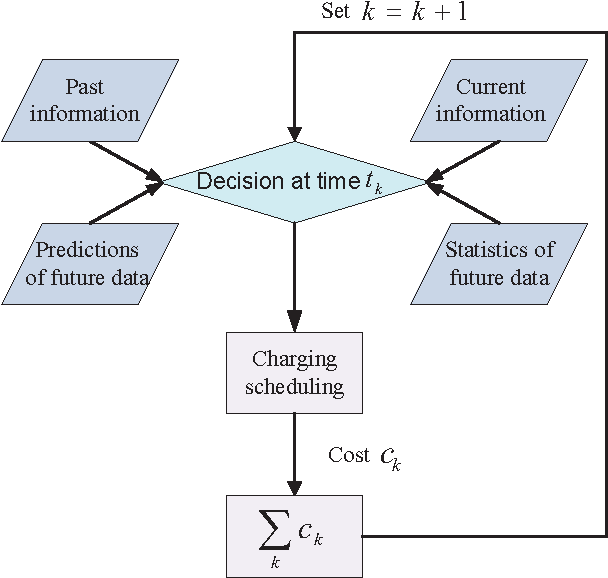
\includegraphics[width=0.7\textwidth]{images/online-algorithms-schedule.png}
%     \centering
%     \caption[Proces dodávania energie pre elektromobily s využitím online plánovacie algoritmov.]{Proces dodávania energie elektromobilom s použiťím online algoritmov. Zdroj obrázka je \cite{Tang2016OnlineCS}.}
%     \label{onlinealg:obrnotyet}
%     \end{figure}
% Obrázok \ref{onlinealg:obrnotyet} ilustruje proces dodávania energie pre elektromobily s využitím online algoritmov. Obrázok hlavne popisuje, na základe čoho sa agregátor flexibility rozhoduje pri prideľovaní energie elektromobilom. 

% \subsubsection*{Porovnanie offline a online algoritmov} Keďže je ťažké získavať informácie o príchode nových elektromobilov (drahé alebo nemožné), tak sa využívajú v praxi prevažne online algoritmy. Offline algoritmy majú viac informácii o budúcich príchodov elektromobilov a preto generujú vyššie dodávky pre elektromobily ako online algoritmy. 

% % opravit prichod buducich elektromobilov na buduce prichody elektromobilov
% \begin{figure}[H]
%     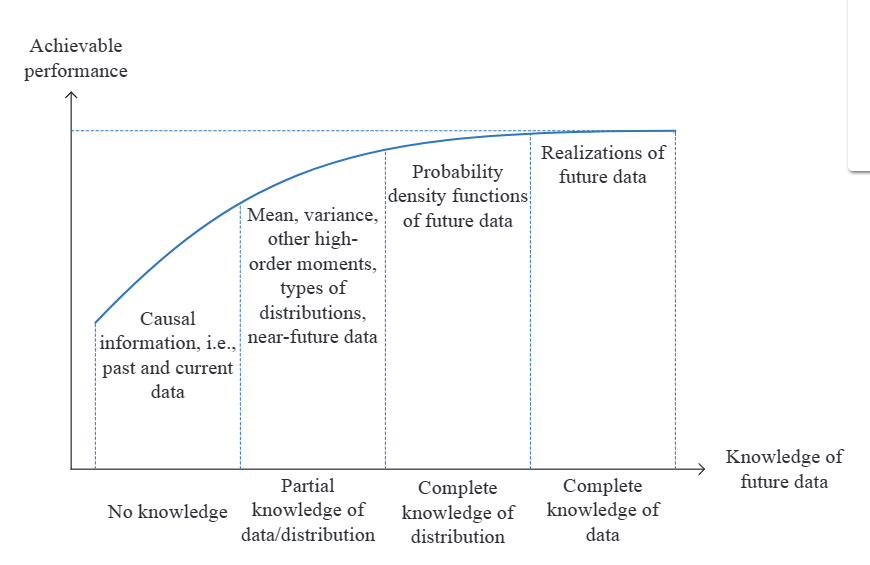
\includegraphics[width=\textwidth]{images/future_knowledge_cars.png}
%     \centering
%     \caption[Vplyv vedomostí o budúcich príchodov elektromobilov na výkonnosť plánovacieho algoritmu.]{Graf ilustrujúci vplyv vedomostí o budúcich príchodoch elektromobilov na výkonnosť algoritmu. Zdroj grafu je \cite{Tang2016OnlineCS}.}.
%     \label{architectureacnsim:obr2}
%     \end{figure}

% \subsubsection*{Náš spôsob riešenia problému} My riešime optimalizačný problém dodania maximálneho množstva energie pre elektromobily pri zachovaní obmedzení nabíjacej siete. Nabíjacia sieť má infraštruktúru a obmedzenia rovnaké ako v článku \cite{lee2021acnsim}. Na riešenie tohoto optimalizačného problému používame online scheduling algoritmy. 
% % V týchto online algoritmoch riešime optimalizačný problém prideľovania maximálnej energie pri zachovaní obmedzení nabíjacej siete.  
% Problém prideľovania maximálnej energie pri zachovaní obmedzení nabíjacej siete riešime viacerými spôsobmi, pomocou linéarneho vyhľadávania, metódy bisekcie a pomocou metódy zlatého rezu. 
% \cite{chen2021smoothed}

% Nižšie uvádzame optimalizačné metódy, ktoré využívame v experimentoch na riešenie optimalizačného problému s využitím online algoritmov.

% % \subsection{Signály}
% % \subsection{Cena nabíjania v čase.}
% % Pomocou podmodulu Signals v ACN portal implementácii vieme zahrnúť dôležité vonkajšie vplyvy nabíjaní, menovite: tarify, krivky solárnych generátorov a 
% \section{Metóda zlatého rezu.}
% % \section{Metóda zlatého rezu}
% %TODO upravit este
% Metóda zlatého rezu sa používa pri riešení problému nájdenia maxima alebo minima unimodálnej funkcie. Unimodálna funkcia je taká, ktorá obsahuje len jedno maximum alebo minimum na intervale $[a, b]$. (zdroj prvy) \cite{} Táto metóda je analogická k optimalizačnej metóde bisekcie. Analogickosť metódy zlátého rezu a metódy bisekcie spočíva v tom, že počiatočný interval $[a, b]$ je nahradený viacerými intervalmi $[a_{i}, b_{i}], i = 2, 3,  \dots$.   \cite{lecture_optimisation} 


% %zdroj 
% % zdroj2 https://www.math.kent.edu/~reichel/courses/intr.num.comp.2/lecture16/lecture8.pdf


% \section{Metóda dichotómie.}
% % \section{Metóda dichotómie}
% %TODO
% Metóda dichotómie rieši jednorozmerné optimalizačné problémy a vieme ju aplikovať len na unimodálne funkcie (unimodálna funkcia, ktorú definujeme na intervale $[a,b]$ má na tomto intervale presne jeden bod, ktorý je maximom alebo minimom funkcie).

% Postup, ktorý metóda dichotómie využíva spočíva z viacerých krokov:
% \begin{enumerate}
%     \item Uvažujme unimodálnu funkciu $f$, ktorá ma na intervale $[a,b]$ minimum alebo maximum.
%     \item  Vygenerujeme dva nové body $c = \frac{a + b}{2} - \epsilon$ a $d = \frac{a + b}{2} - \epsilon$. Platí, že $\epsilon > 0$ a $2 \cdot \epsilon < (a - b)$.  
%     \item Skontrolujeme, či $f(c) > f(d)$ alebo $f(c) < f(d)$. Ak platí $f(c) > f(d)$, tak dostaneme nový interval $[a, b] = [a, d]$. Inak $[a, b] = [c, b]$. % skontrolovat este 
% \end{enumerate}
% Kroky $2$ a $3$ metóda dichotómie opakuje dokým  nenájde riešenie. 
% Metóda dichotómie nájde riešenie vtedy, keď nový interval bude dostatočne malý (menší než epsilon).

% Vyriešime optimalizačný problém pomocou viacnásobného zmenšenia intervalu $[a, b]$ o polovicu.




% \section{Metóda rovnomerného delenia intervalu.}
% \section{Metóda rovnomerného delenia intervalu}
%TODO





% TODO: premiestnit algoritmy, ktore neimplemetujem do sucasneho stavu riesenia problematiky v prvej kapitole 


% \section{Neriadené nabíjanie.}
% Tento plánovací algoritmus prideľuje každému elektromobilu maximálne množstvo energie a pritom neberie do úvahy obmedzenia infraštruktúry nabíjacej stanice. Toto je najjednoduší typ nabíjania, ktorý je stále používaný vo väčšine nabíjacích systémov na svete. \cite{lee2021acnsim}

% %rad <-> front 
% %TOTO implementovat aby som tomu pochopil a mozno prepisat 
% \section{Round Robin.}
% % \subsection{Round Robin (RR).}
% Plánovací algoritmus Round Robin, ktorý nazývame skrátene RR je algoritmus, ktorý je založený na myšlienke zdieľania nabíjacej kapacity medzi všetkými aktívnymi elektromobilmi. Pre každý aktívny elektromobil kontroluje algoritmus dve podmienky:
% % mozno otazky do uvodzoviek
% \begin{enumerate}
%     \item Je možné zvýšiť nabíjanie o 1kWh tak, aby sme zachovali obmedzenia nabíjacej siete? Ak áno, tak nabijeme elektromobil so zvýšenou rýchlosťou nabíjania a následne elektromobil pridáme na koniec radu.
%     \item Nie je možné zvýšiť nabíjanie o 1kWh tak, aby sme zachovali obmedzenia nabíjacej siete? Ak áno, tak nabijeme elektromobil s fixným nabíjaním. Elektromobil necháme vo radu na rovnakom mieste.
%     % To znamená, že vozidlo nabíja dovtedy, keď bude možné rýchlosť nabíjania elektrického vozidla zvýšiť.
% \end{enumerate}
% Elektromobily, ktoré dostali požadovanú energiu sú z radu odstránené. Algoritmus RR skončí vtedy, keď v rade nebude žiaden elektromobil. \cite{lee2021acnsim}

% \begin{figure}[H]
%     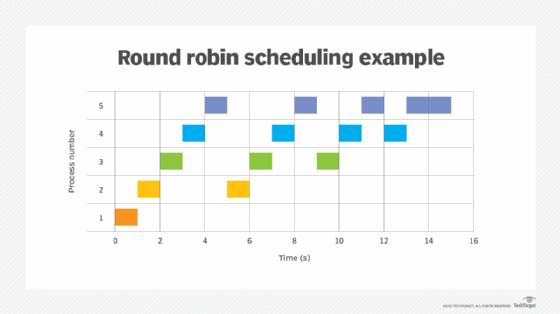
\includegraphics[width=\textwidth]{images/round-robin-example.png}
%     \centering
%     \caption[Príklad plánovacie algoritmu Round Robin v praxi.]{Prideľovanie času procesom na základe plánovacieho algoritmu Round Robin. Každý spotrebiteľ má prístup k rovnakým zdrojom pomocou algoritmu Round Robin. Zdroj obrázka: \cite{websitecroundrobin2023}.}
%     \label{architectureacnsim:obr2}
%     \end{figure}

% Príklad:
% \UNFIN
% % 

%pozriet ci je taky nazov v anglictine

% \section{Triediace plánovacie algoritmy}
% Triediace plánovacie algoritmy, ktoré spomíname v tejto sekcii prideľujú energiu elektromobilom v takom poradí, v akom tie elektromobily utriedili. Trediace plánovacie algoritmy triedia elektromobily na základe jedného parametra alebo viacerých parametrov. 

% %stanice vs siete zjednotit
% Následne na riešenie problému maximálneho pridelenia energie elektromobilu pri zachovaní obmedzení nabíjacej siete využívajú triediace plánovacie algoritmy metódu bisekcie alebo iných metód (napr. metóda lineárneho vyhľadávania). Pre každý elektromobil sa vyrieši tento problém jednotlivo a algoritmus postupne pridelí energiu elektromobilom.


% Tieto algoritmy môžu byť implementované ako online, a aj ako offline algoritmy. V prípade offline verzie triediacich plánovacích algoritmov vieme lepšie minimalizovať cenu ako v online plánovacích algoritmoch. \cite{chen2021smoothed}

% \subsection{Least Laxity First.}
% % \subsubsection{Least Laxity First (LLF)}
% Algoritmus Least Laxity First (skrátene nazývame LLF), je triediaci plánovací algoritmus, ktorý prideľuje elektromobilom energiu v poradí od elektromobilu s najnižšiou laxitou po elektromobil s najvyššou laxitou. Nevýhodou triediaceho plánovacieho algoritmu LLF je, že spôsobuje veľké výkyvy v rýchlosti nabíjania pri nabíjaní elektromobilov. Napríklad, keď príde veľa elektromobilov, ktoré majú ešte nižšiu laxitu ako pôvodný elektromobil s najnižšiou laxitou, tak sa môže stať, že pôvodnému elektromobilu sa nepridelí žiadna energia alebo málo energie. Dlhodobo, taký spôsob nabíjania s výkyvmi v rýchlosti nabíjania môže skrátiť životnosť batérii elektromobilov.\cite{chen2021smoothed}


% % zdroje 30,31,32 niekde by mala by byt implementacia asi 32
% Laxitu počítame na základe vzorca:
% \begin{equation}
%     \text{Laxita} = \text{zostávajúci čas do odchodu} - \frac{\text{zostávajúca požadovaná energia}}{\text{rýchlosť nabíjania}},
% \end{equation}
% kde predpokladáme, že rýchlosť nabíjania je vždy konštantná.

% \subsubsection*{Príklad}
% Každý elektromobil $i$ má definovanú trojicu $(a_{i},d_{i},e_{i})$, kde $a_{i}$ je čas pripojenia elektromobilu na nabíjačky, $d_{i}$ je čas odpojenia vozidla z nabíjačky a $e_{i}$ je požadovaná energia.  
% Máme $4$ vozidlá ktoré majú nasledujúce parametre:
% \begin{enumerate}
%     \item (9, 15, 4).
%     \item (9, 12, 1).
%     \item (12, 17, 4).
%     \item (9, 13, 3).
% \end{enumerate}
% Zároveň máme 4 nabíjačky v nabíjacej stanici, a preto vieme zabezpečiť nabíjanie vozidiel kedykoľvek, bez použitia prioritnej fronty. Predpokladáme, že cena energie je konštantná. Zvoľme rýchlosť nabíjania každej stanice na $1$. Obmedzenia nabíjacej siete sú, že môže každú hodinu dodať len $2Kw$ energie.

% Naša úloha je nájsť optimálny scheduling, kde našim cieľom je zabezpečiť požadované množstvo energie pre všetky elektromobily. \\

% Náš optimálny scheduling problému je: \\
% % \begin{center}
% \begin{tabular}{ |c|c|c|c|c|c|c|c| }
%    \hline
%     & t = 9 & t = 10 & t = 11 & t = 12 & t = 14 & t = 15 & t = 16 \\
%    \hline
%    Vozidlo 1  & 1  & 0 & 1 & 1 & 1 & - & - \\
%    Vozidlo 2  & 0  & 1 & 0 & - & - & - & - \\
%    Vozidlo 3  & -  & - & - & 1 & 1 & 1 & 1 \\
%    Vozidlo 4  & 1  & 1 & 1 & 0 & - & - & - \\
%   \hline
% \end{tabular}  \\
% % \end{center}

% Ak napríklad vymeníme nabíjanie vozidla 2 o 10:00 s nabíjaním vozidla 1, tak nám vzniká iný scheduling, ktorý je tiež optimálny.

% Na druhej strane existuje aj neoptimálny scheduling tohoto príkladu, vypojením vozidla 3 o 12:00. Vozidlo 3 v tom prípade by sa vypojilo z nabíjacej siete buď o 9:00, 10:00 alebo 11:00 a napojilo o 12:00.


% \subsection{Smoothed Least Laxity First.}
% % \subsection{Smoothed least laxity first.}
% Smoothed Least Laxity First (skrátene sLLF) je triediaci plánovací algoritmus založený na algoritme LLF. Tento algoritmus lepšie rieši optimalizačný problém prideľovania maximálnej energie elektromobilom pri zachovaní obmedzení infraštruktúry nabíjacej siete lepšie ako algoritmus LLF. Algoritmus sLLF zároveň neobsahuje veľké výkyvy v rýchlosti nabíjania pri prideľovaní energie elektromobilom na rozdiel od algoritmu LLF.

% % skontrolovat notaciu
% Popis algoritmu sLLF sa nachádza v článku \cite{chen2021smoothed}.
% % Laxitu v tomto algoritme budeme počítať odlišne, než v bežnom LLF, takto:
% % \begin{equation}
% %     l_{i}(t) = [d_{i} - t]^{+} - \frac{e_{i}(t)}{\overline{r_{i}}}.
% \end{equation}
% Keďže pri našej implementácii máme k dispozícii len aktívne elektrické vozidlá, tak pre tie vozidlá, ktoré ešte neprišli laxitu nepočítame.

% Pre prípad $t < d_{i}$ počítame $l_{i}(t + 1)$ takto:
% \begin{gather*}
%     l_{i}(t + 1) = [d_{i} - (t + 1)]^{+} - \frac{e_{i}(t + 1)}{\overline{r_{i}}}. \\
%     l_{i}(t + 1) = [d_{i} - t]^{+} - 1 - \frac{e_{i}(t + 1)}{\overline{r_{i}}}. \\
%     l_{i}(t) +  \frac{e_{i}(t)}{\overline{r_{i}}} = [d_{i} - t]^{+}. \\
%     l_{i}(t + 1) = l_{i}(t) +  \frac{e_{i}(t)}{\overline{r_{i}}} - 1 - \frac{e_{i}(t + 1)}{\overline{r_{i}}}.
% \end{gather*}
% Kde $e_{i}(t + 1) - e_{i}(t) = r_{i}(t)$ (Množstvo dodanej energie za čas $t$), tým dostaneme:

% \begin{gather*}
%     l_{i}(t + 1) = l_{i}(t) - 1 - \frac{r_{i}(t)}{\overline{r_{i}}}.
% \end{gather*}



% Druhý krok algoritmu je maximalizácia minimálnej laxity medzi všetkými elektrickými vozidlami.

% \UNFIN

% Výpočtová zložitosť tohoto algoritmu je $O(V + log(\frac{1}{\delta}))$, kde V je počet aktívnych elektromobilov a $\delta$ je level tolerovateľnej chyby. \cite{chen2021smoothed}

% \subsection{Enhanced Least Laxity First.}
% Ako reakciu na problém oscilácie pri nabíjani elektromobilov v algoritme LLF vzniklo mnoho variánt vylepšeného algoritmu LLF. Jedným z nich je Enhanced Least Laxity First (ELLF). Algoritmus ELLF zaradí elektromobily s rovnakou najnižšiou laxitou do jednej skupiny. Potom algoritmus ELLF pridelí energiu elektromobilom v skupine použitím  scheduling algoritmu EDF. Na pridelenie energie zvyšku elektromobilov algoritmus ELLF aplikuje LLF. \cite{websiteenhancedllf}

% \subsection{Earliest Deadline First.}
% % \subsubsection{Early deadline first (EDF).}
% % \subsubsection{Early deadline first (EDF)}
% Algoritmus Early deadline first skrátene nazývame EDF, je triediaci plánovací algoritmus. Algoritmus EDF prideľuje energiu elektromobilom v poradí od elektromobilov s najskorším časom odchodu po elektromobily s najneskorším časom odchodu. \cite{lee2021acnsim}



% \subsection{Group Earliest Deadline First.}
% % \subsection{Group earliest deadline first (EDF).}
% Algoritmus Group Earliest Deadline First je plánovací algoritmus, ktorý vytvorili zo zámerom zlepšenia výkonnosť algoritmu EDF počas preťaženia reálnej multimediálnej aplikácie. Tento schedling algoritmus sa zakladá na myšlienke skupinového schedulingu. To znamená, že elektromobily, ktoré majú podobné časy príchodu patria do skupiny. Potom sa priraďuje energia týmto elektromobilom na základe scheduling algoritmu Shortest Job First. \cite{comparisonofalg}

%pozri ci rovnake casy elektromobilov - pozri definiciu este raz!!!


% \subsection{Group priority earliest deadline first (EDF).}

% \cite{comparisonofalg}



% Máme 5 vozidiel.




% \subsection{First-Come First-Served.}
% % \subsection{First Come First Served}
% Triediaci plánovací algoritmus First-Come First-Served (skrátene FCFS) má veľmi podobnú funkcionalitu ako algoritmus neriadeného nabíjania. Hlavný rozdiel spočíva v tom, že algoritmus FCFS je časovo oneskorený, lebo obsahuje elektromobily v rade, takže každý elektromobil si musí počkať pre svoje nabíjanie. \cite{lee2021acnsim}


% %TOTO pozriet ci nemyslia skor arrival time nez connection time
% \subsection{Last-Come First-Served.}
% % \subsection{Last Come First Served}
% Triediaci plánovací algoritmus Last-Come First-Served (skrátene LCFS) priraďuje energiu elektromobilom, prioritne od vozidla s najneskorším časom pripojenia na nabíjačku po vozidlo s najskorším časom pripojenia na nabíjačku. \cite{lee2021acnsim}

% \subsection{Longest Remaining Processing Time.}
% % \subsection{Longest remaining processing time}
% Triediaci plánovací algoritmus Longest Remaining Processing Time je algoritmus, ktorý prideľuje energiu elektromobilom takto:
% \begin{enumerate}
%     \item Utriedi vstupné pole aktívnych elektromobilov, a to od elektromobilu s najdlhším zostávajúcim časom nabíjania po elektromobil s  najkratším zostávajúcim časom nabíjania.
%     \item Pre každý elektromobil v tom poradí algoritmus vyrieši optimalizačný problém prideľovania maximálnej energie pri zachovaní obmedzení infraštruktúry. 
% \end{enumerate}


% \subsection{Shortest Job Next.}
% % \subsection{Shortest job next}
% Algoritmus Shortest Job Next, skrátene SJN je trediaci plánovací algoritmus. SJN funguje ako Longest Remaining Processing Time až na jeden rozdiel, ktorý spočíva v tom, že pole aktívnych elektromobilov triedi od  elektromobilu s najkratším zostávajúcim časom nabíjania, po vozidlo s najdlhším zostávajúcim časom nabíjania.

% % \section{Kontrolné algoritmy}
% % % \section{Kontrolné plánovacie algoritmy}

% % V tejto sekcii hovoríme o kontrolných algoritmoch, ktoré riešia optimalizačný problém pridelenia maximálneho množstva energie elektromobilom pri zachovaní obmedzení infraštruktúry. Kontrolné algoritmy sú algoritmy, ktoré poskytujú kontrolné akcie na základe vstupných dát, za účelom zistenia konkrétneho cieľa (...). 
% % %TODO lepsie popisat
% % Bez kontrolných algoritmov by nemohli fungovať automatické systémy, ktoré v súčastnosti využívame. 
% % %ake automaticke systemy??
% % Tieto algoritmy musia vedieť fungovať v obmedzenom prostredí, ako napríklad pri obmedzeniach uvedených v sekcii \ref{vych:konfaobmedzenia}. \cite{websitecontrolalg2023}

% % \subsection{Typy kontrolných algoritmov}


% % \subsubsection*{open-loop algoritmy} Sú najjednoduším typom kontrolných algoritmov, ktoré vracajú pre rovnaký vstup rovnaký výstup. Používaju sa v systémoch, kde netreba meniť výstupné dáta na základe zmeny vstupných dátach.


% \subsubsection*{closed-loop algoritmy} Sú zložitejšie než open-loop algoritmy, ktoré používajú odozvu s cieľom úpravy výstupných dát na základe zmien vstupných dát. Používajú sa v systémoch, kde sa výstup musí upravovať na základe zmien vo vstupe.

% \subsubsection*{feedback-control algoritmy} Sú najzložitejším typom kontrolných algoritmov, ktoré používajú odozvu s cieľom úpravy výstupných dát na základe zmien vstupných dát. Používaju taktiež prediktívne modely aby predpovedali zmenu vo vstupných dátach. Používajú sa v systémoch, ktoré predpovedajú budúce zmeny vstupov, a kde sa výstup  musí upravovať na základe zmien vo vstupe.
% \cite{websitecontrolalg2023}
% \subsection{Model Predictive Control.}
% % \subsection{MPC}
% % mam nazov algoritmu prelozit do slovenciny, aj ked sa pouziva bezne pod anglickym nazvom???
% Model Predictive Control skrátene MPC je jeden z kontrolných algoritmov. MPC je kontrolný algoritmus založený na odovzve. MPC využíva prediktívny model, aby zistil kontrolné akcie v budúcnosti, ktoré optimalizujú výkon počas stanoveného časového horizontu. Cieľom MPC je zabezpečiť čo najlepšie kontrolné akcie, a pritom spĺňať obmedzenia nabíjacej siete.

% \subsubsection*{Komponenty MPC} MPC sa skladá z 3 komponentov:

% \begin{enumerate}
%     \item Matematický model procesu. Tento matematický model zachytáva vzťah medzi vstupom a výstupom a zahŕňa aj dynamiku systému.
%     \item Optimizátor, ktorý rieši zadaný optimalizačný problém a pritom spĺňa obmedzenia systému.
%     \item Funkcia nákladov, ktorá meria kvalitu riešenia optimizátora. 
% \end{enumerate}



% \subsubsection*{Výhody použitia MPC} Veľká výhoda kontrolného algoritmu MPC v porovnaní s tradičnými kontrolnými algoritmami je, že nemusí mať fixný počet kontrolných parametrov, ktoré sú potom upravované na základe experimentov. Algoritmus MPC využíva dynamický model, aby predikoval správanie v budúcnosti. MPC na rozdiel od tradičných kontrolných algoritmov vie riešiť aj nelineárne kontrolné problémy. Nelineárne kontrolné problémy sú problémy, v ktorých je vzťah medzi vstupnom a výstupom nelineárny (nevieme ho vyjadriť pomocou lineárnej funkcie). \cite{websitecontrolalgMPC2023}
% % lepsie popisat nelinearny


% \subsubsection*{Existujúce riešenia} Veľa existujúcich riešení problému hľadania optimálneho schedulingu využíva algoritmus MPC. My sa orientujeme hlavne na algoritmus nazývaný adaptívný algoritmus nabíjania,
% %Adaptive Charging Algorithm pozriet ci nie je lepsi preklad
% ktorý je založený na MPC a rieši problém konvexnej optimalizácie. \cite{lee2021acnsim,lee2021adaptivephd}

% \UNFIN




% \subsection{Penalised Predictive Control.}
% Algoritmus Penalised Predictive Control (PPC) je vylepšená verzia algoritmu MPC. Zmysel algoritmu spočíva v komunikácii medzi systémovým operátorom a agregátorom. Agregátor poskytne flexibilitu (naučenú na základe RL algoritmu SAC) systémovému operátorovi. Systémový operátor aplikuje algoritmus PPC, ktorého vstupom je flexibilita a výstupom je množstvo energie. Následne systémový operátor pridelí výstupnú energiu algoritmu PPC agregátorovi. Agregátor potom použije jednoduchý plánovací algoritmus (EDF alebo LLF), aby pridelil túto energiu aktívnym elektromobilom. Tento proces sa opakuje pre každú časovú jednotku.

% Na rozdiel od MPC algoritmu nevyžaduje PPC algoritmus veľa premenných, ale na druhej strane obsahuje obsiahly algoritmus SAC na učenie flexibility. Výhodou algoritmu PPC je, že nemusí vedieť o obmedzeniach siete a stavu pri riešení optimalizačného problému, lebo sú zahrnuté vo flexibilite generovanej agregátorom. \cite{Li_2021}


% \begin{figure}[H]
%     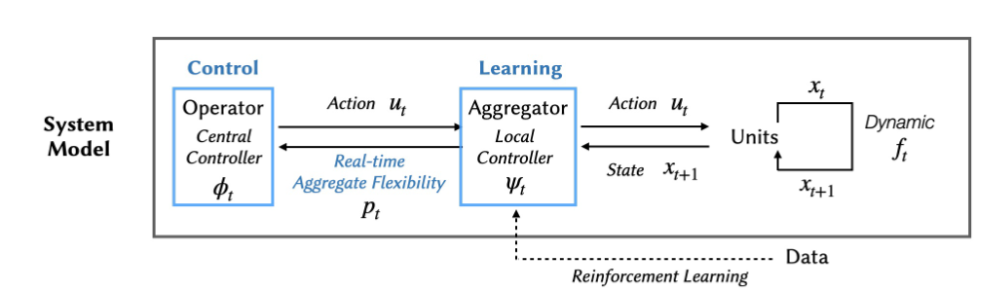
\includegraphics[width=\textwidth]{images/systemmodel.png}
%     \centering
%     \caption[Model systému, využívajúci PPC.]{Model systému, ktorý je  sa používa v PPC. Operátor implementuje kontrolný algoritmus a agregátor implementuje RL algoritmus, ktorý generuje flexibilitu. 
%     Obrázok je prevzatý z \cite{Li_2021}.}
%     \label{architectureacnsim:obr2}
%     \end{figure}

% ~\eqref{eq:current}
% \section{Cena nabíjania.}
% Náš spôsob definovania ceny nabíjania je: na konci každého mesiaca nastavíme ceny nabíjania ako $\alpha_{t}^{*}$, pre každé nabíjanie $i$ v tom mesiaci. Hovoríme, že $e_{i}$ je dodaná energia pre spotrebiteľa $j$ počas nabíjania $i$, kde $S_{j}$ je množina všetkých nabíjaní používateľa $j$. Potom náklady za nabíjanie spotrebiteľa $j$ sa na konci mesiaca vypočítajú takto:
% \begin{equation}
%     \sum_{i \in S_{j}}  \alpha_{i}^{*}e_{i}. 
% \end{equation}
% Narozdiel od konštantných cien a cien závislých na čase (napríklad v \cite{Li_2021}) my používame ceny (tarify), ktoré zachytávajú skutočné ceny energie. Skutočné ceny energie závisia od jej dopytu a od preťaženie infraštruktúry.  \cite{evpricingsystem}
% %TODO poslednu vetu mozno treba upravit taktiez este raz skontrolovat prve vety a vzorec


% \begin{figure}[H]
%     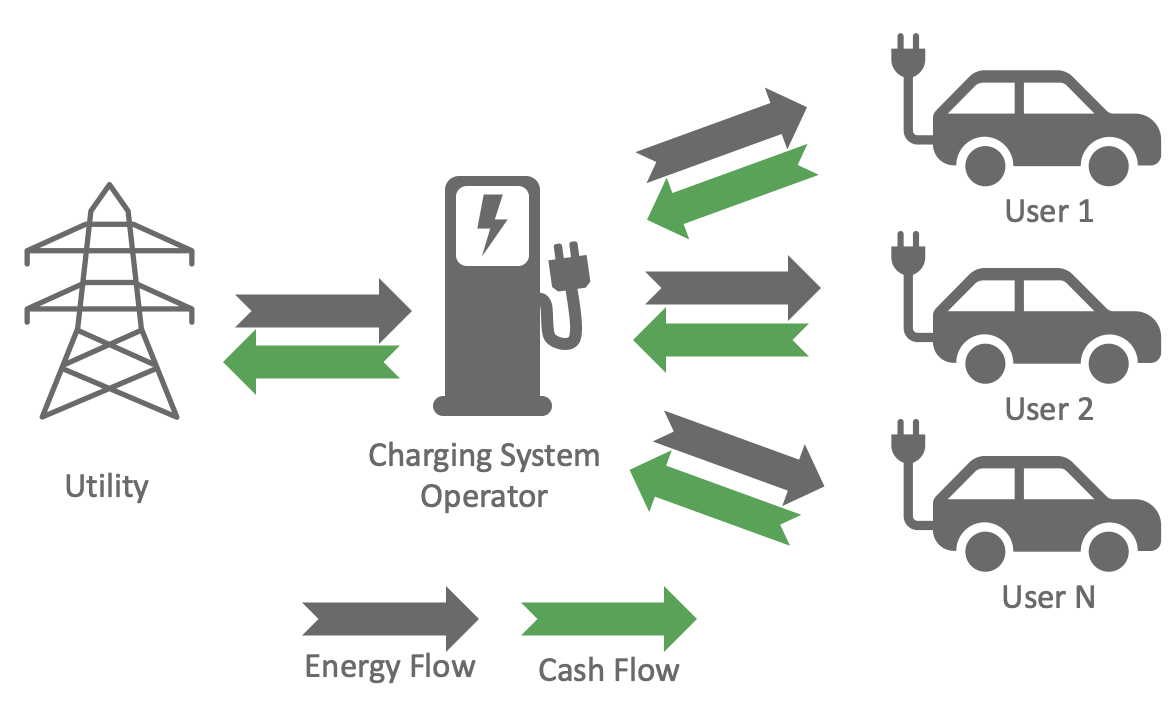
\includegraphics[width=\textwidth]{images/energy_flow_costs.png}
%     \centering
%     \caption[Systém toku energie a ziskov.]{Systéme toku energie a aj zisky za energiu. Zdroj obrázka je: \cite{websitpricecharging2023}.}
%     \label{architectureacnsim:obr2}
%     \end{figure}
%TODO lepsie popisat asi co to utilita a charging operator je mozno to trbea najst

% na základe ktorého vie potom agregátor flexibility vie prideliť energiu elektrickým vozidlám tak, aby sme optimalizovali tok energie a minimalizovali naše náklady na kapacitu a minimalizovali náklady spotrebiteľov.
% \section{Least Laxity First} 


% \section{Smoothed Least Laxity First.}

% \section{Riešenie našeho problému.}

% \section{Návrh našeho MPC modelu.}


% Náš triediaci algoritmus sa nazýva Least Laxity First (ďalej len LLF). LLF pre každého používateľa $j$ vypočíta jeho laxitu použitím vzorca 

% \begin{eqnarray}
%     laxita = d_{t}(j) - \frac{e_{t}(j)}{r(j)},
% \end{eqnarray}
% kde $d_{t}(j)$ je zostávajúci čas na nabíjanie a $e_{t}(j)$ je zostávajúca požadovaná energia v čase $t$). Na základe vyššie vypočítanej laxity utriedi používateľov do prioritného frontu, kde používatelia s najnižšiou laxitou budú preferovaní. 


% Potom, keď už každý spotrebiteľ má vypočítanú vlastnú laxitu, tak algoritmus prideľuje elektrickú energiu (aj nulovú) v každom čase $t$ spotrebiteľom s najmenšou laxitou po najväčšiu laxitu. 
% % Zo vzorca vieme určiť, že autá, ktoré odchádzajú skoršie a prípadne chcú nabiť viac energie majú menšiu laxitu.

% % 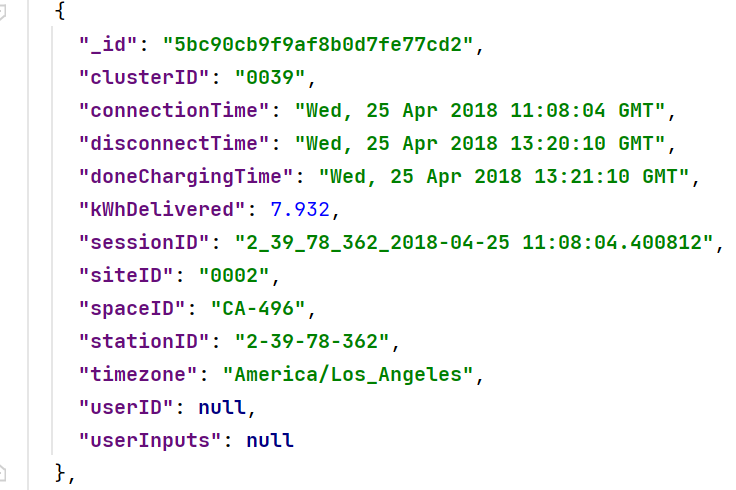
\includegraphics{images/acndata.png}


% % \section{Logika prvého rádu}

% % \subsection{Jazyk logiky prvého rádu}

% \subsection{Semitermy a semiformuly}

% \aDpF{A} je hĺbka formuly $A$

% \aSubst{A}{x}{t} je substitúcia

% \subsection{Termy a formuly}

% \subsection{Henkinove konštanty a Henkinove axiómy}

% \aHc{A} je Henkinova konštanta

% $A\aReplace{r}{s}$ je hlboké nahradenie (deep replacement)

% \section{Sekventový kalkulus \nLKh}

% \subsection{Multimnožiny}

% \subsection{Sekventy}

% \subsection{Odvodzovacie pravidlá}

% \begin{prooftree}
% \AxiomC{\phantom{$S_1$}}
% \RightLabel{,}
% \UnaryInfC{$S$} 
% \DisplayProof
% \qquad
% \AxiomC{$S_1$}
% \RightLabel{,}
% \UnaryInfC{$S$} 
% \DisplayProof
% \qquad
% \AxiomC{$S_1$}
% \AxiomC{$S_2$}
% \RightLabel{,}
% \BinaryInfC{$S$}
% \end{prooftree}

% \begin{list}{}{\setlength{\leftmargin}{0in}\setlength{\rightmargin}{0in}}

% \item \emph{Axioms}

% \begin{prooftree}
% \AxiomC{}
% \LeftLabel{\nAx}
% \RightLabel{($A$ is atomic),}
% \UnaryInfC{$A, \Gamma \fCenter \Delta, A$} 
% \DisplayProof
% \quad
% \AxiomC{}
% \LeftLabel{\nLf}
% \RightLabel{,}
% \UnaryInfC{$\nF, \Gamma \fCenter \Delta$}
% \DisplayProof
% \quad
% \AxiomC{}
% \LeftLabel{\nRt}
% \RightLabel{.}
% \UnaryInfC{$\Gamma \fCenter \Delta, \nT$}
% \end{prooftree}

% \item \emph{Propositional rules}

% \begin{prooftree}
% \AxiomC{$¬A, \Gamma \fCenter \Delta, A$}
% \LeftLabel{\nLn}
% \RightLabel{,}
% \UnaryInfC{$¬A, \Gamma \fCenter \Delta$}
% \DisplayProof\quad
% \AxiomC{$A, \Gamma \fCenter \Delta, ¬A$}
% \LeftLabel{\nRn}
% \RightLabel{,}
% \UnaryInfC{$\Gamma \fCenter \Delta, ¬A$}
% \end{prooftree}

% \item \emph{Structural rules}

% \begin{prooftree}
% \AxiomC{$\Gamma \fCenter \Delta, A$}
% \AxiomC{$A, \Gamma \fCenter \Delta$}
% \LeftLabel{\nCut}
% \RightLabel{.}
% \BinaryInfC{$\Gamma \fCenter \Delta$}
% \end{prooftree}

% \end{list}

% \subsection{Dôkazy}

% \(
% \pi \rProof \Gamma \fCenter \Delta
% \)

% \aHtP{\pi} je hĺbka dôkazu $\pi$

% \aCrP{\pi} je rezová hodnosť dôkazu $\pi$
